% ================================================================
% Use the following if all authors are from the SAME institution
% ================================================================
\documentclass[accepted,single]{gipaper}

% use Times fonts
\usepackage{times}
% make sure English hyphenation rules, etc. loaded
\usepackage[english]{babel}
% permits inclusion of PNG, JPG, and PDF files under pdflatex
\usepackage{graphics}

% permits figures at bottom of page
\usepackage{dblfloatfix}

\usepackage{epsfig}
\usepackage{newalg}

% \usepackage{url}
% \bibliographystyle{IEEEtran.bst}

% a more flexible replacement for "verbatim" for typesetting pseudocode
\usepackage{alltt}
% gives automatic table of contents, permits setting PDF
% attributes of document.   Set page size in pdftex.cfg file;
% the "letterpaper" option to hyperref is unreliable...
\usepackage[
    pdftitle = "{Dynamic Bandwidth Allocation with Minimum Rate Guarantees Using OpenFlow}",
    pdfauthor = "{Joel van Egmond}"
]{hyperref}

\title{Dynamic Bandwidth Allocation with Minimum Rate Guarantees Using OpenFlow}

\newauthor{mm}{Joel van Egmond}{}
% Can add more authors
%\newauthor{se}{Someone Else}{}
%\newauthor{ya}{Yet Another}{}
%\newauthor{fa}{Fourth Author}{}

% Common affiliation
\affiliation{
    Department of Computer Science \\
    University of Calgary
}

% ================================================================
% Use the following if the authors are from MULTIPLE institutions
% ================================================================
%
% \documentclass[accepted,oneeach]{gipaper}
% \usepackage{graphics}
% \usepackage{hyperref}
%
% \title{Paper Format for CPSC 502/503/601 \\ Instructions to Authors}
%
% \newauthor{wd}{Author One}{Department of Computing Science\\ University of Nowhere}
% \newauthor{se}{Someone Else}{Another Department\\ A Company}
% \newauthor{ya}{Yet Another}{Yet Another Department\\ Another University}
% \newauthor{fa}{Fourth Author}{Department of Computing Science\\ University of Nowhere}
%
% ================================================================
% The rest of the document follows.
% ================================================================

\abstract{ Quality of Service (QoS) control typically refers to network mechanisms used to guarantee a certain service from the network \cite{Krishna:2016}. Many service providers use hard QoS controls to guarantee bandwidth to their clients. In current solutions excess idle bandwidth is wasted, but with the emergence of Software-Defined Networking (SDN) and the OpenFlow protocol, it is possible to program a network to respond to this problem cheaply and efficiently.
This paper describes the design of an SDN/OpenFlow solution that ensures minimum bandwidth guarantees for clients while fairly distributing the excess bandwidth among current users to maximize link capacity utilization.  }

\begin{document}
\begin{keywords}
OpenFlow, Ryu, software defined networking, traffic shaping, quality of service.
\end{keywords}

%------------------------------------------------------------------
% Introduction
%------------------------------------------------------------------
\section{Introduction}
\label{intro}

Quality of Service (QoS) control typically refers to network mechanisms used to guarantee a certain service from the network \cite{Krishna:2016}. Minimum bandwidth is a service frequently guaranteed by QoS. Internet service providers (ISPs) are common users of QoS technology. Traditional ISPs such as Bell, Telus, and Shaw aim to maximize profits and avoid having excess unused bandwidth by overselling their channel to more clients than it can support, with the assumption that not all clients will be using the channel simultaneously. In contrast, many other large-scale service providers, such as the research and education focused Cybera, ORION, and MRnet do not oversell their channel, opting to use QoS controls to guarantee clients that their allocated bandwidth will always be available even if every single other client is currently using their own maximum allocated bandwidth. Consequently, these networks often have significant amounts of excess idle bandwidth, since it is very unlikely that every client will always be using the network. Currently the bandwidth is wasted while the operation and maintenance costs of the full channel must still be paid. This leads to the problem of how to make use of all this excess bandwidth, while still maintaining the minimum bandwidth guarantees demanded by the clients.

Software-Defined Networking (SDN) is an emerging network paradigm that decouples the network control and forwarding functions, enabling network control to be directly programmable \cite{opennetworking}. This is done by implementing the network control function in a centralized controller node, which communicates to all the network devices in the network through a standardized protocol. OpenFlow is one such protocol, an open standard protocol that acts as an abstracted southbound API to allow the SDN controller to control the routers/switches in its domain \cite{sdx}.

The purpose of the proposed research is to design and implement an SDN solution to the excess bandwidth problem, in order to maximize the utilization of a network while providing minimum bandwidth guarantees to its clients. This will be done by directing network traffic through an OpenFlow enabled switch. The switch will be connected to a SDN controller device, which will use the switch's features to guarantee minimum bandwidths while dynamically allocating the excess bandwidth to clients according to a selection of different algorithms. The algorithms in question are inspired by common CPU scheduling algorithms, but will be custom designed to approximate the functionality of their inspirations within the limitations of the OpenFlow switch environment.

The proposed research will contribute to the body of QoS research by presenting an original SDN/OpenFlow traffic shaping design, which will provide both minimum bandwidth as a guaranteed service, as well as the ability to utilize and fairly distribute the excess bandwidth in the channel. Once implemented the solution will be evaluated first on its ability to guarantee minimum rates, and then on each algorithm's link capacity utilization and fairness of allocation.

% this figure has to be declared here for some reason or it appears on the wrong page
%\begin{figure*}[!b]
%	\centering
%	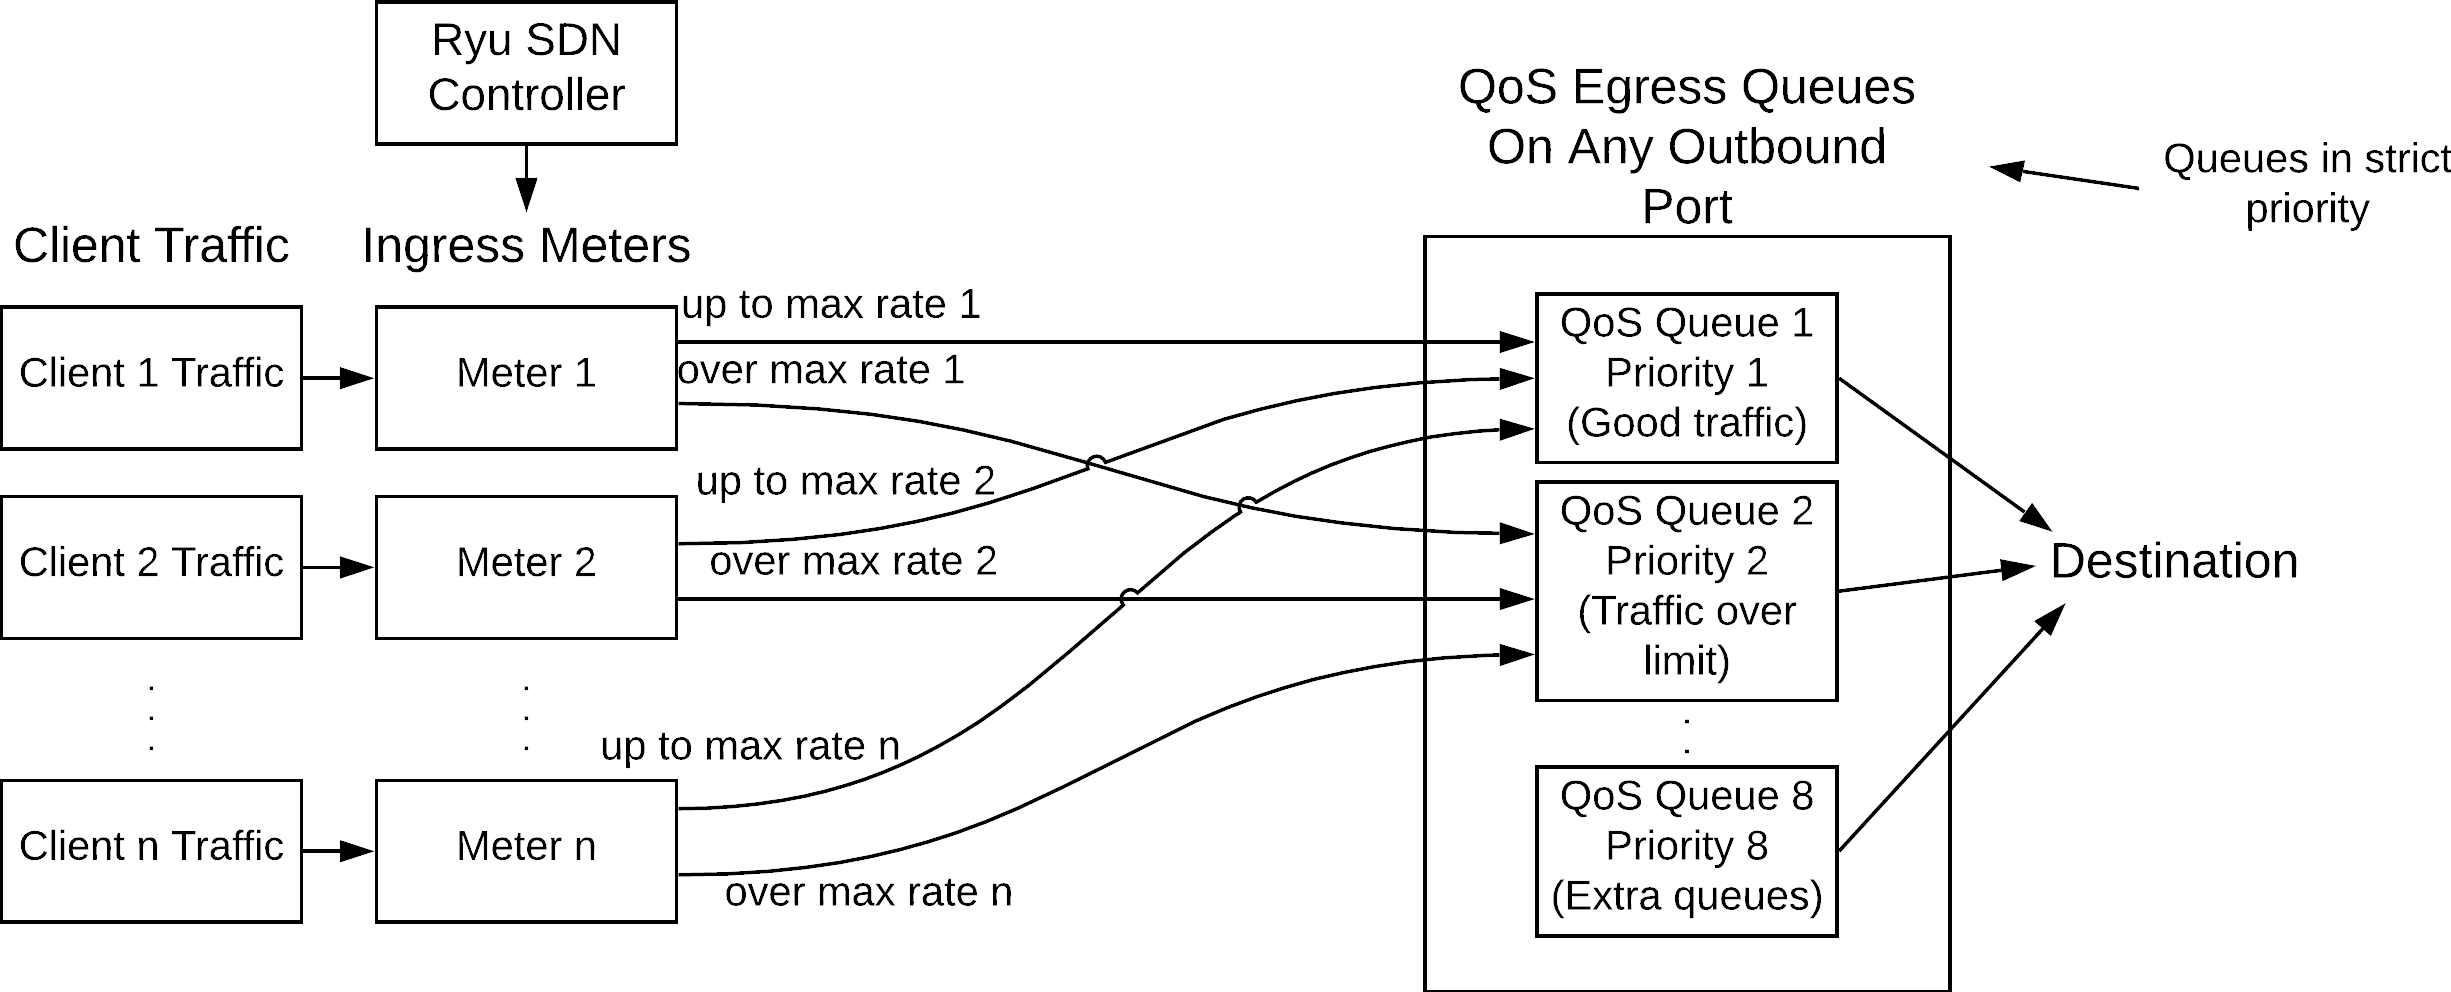
\includegraphics[width=6in]{figs/bwGuar3.png}
%	\caption{ Pica8 setup for minimum bandwidth guarantee. } \label{bwDiag}
%\end{figure*}

\subsection{Key Definitions}
\label{definitions}

yeet whats a METER whats a METER BAND whats a FLOW whats DSCP remark whats a QUEUE

%------------------------------------------------------------------
% Previous Work
%------------------------------------------------------------------
\section{Previous Work}
\label{prev_work}

Previous work that has been conducted relating to this project is focused various methods of using OpenFlow enabled switches to obtain minimum bandwidth guarantees. These focused on two main paradigms: hard guarantees and soft guarantees \cite{softqos}. A hard bandwidth guarantee uses a static reservation of network resources for the specified traffic, whereas a soft bandwidth guarantee uses a differentiated service approach with no reservation, in which some traffic is given priority over other traffic using only currently available network resources. 

\subsection{Hard Guarantee}
\label{prev_hard_qos}

In a 2014 paper, Tomovic et al. \cite{Tomovic:2014} proposed a system with hard QoS guarantees using OpenFlow. The hard guarantee is established by forcing all flows to request bandwidth on the link. The SDN controller evaluates each request and allocates bandwidth to the requesting flow if there is capacity on the link, otherwise the request is rejected. Once allocated, the bandwidth is reserved for exclusive use by that flow until the flow expires. The guarantee is implemented on the switch level by installing an egress queue with minimum and maximum bandwidth equal to the guaranteed bandwidth.

In a later paper, Dwarakanathan et al. \cite{Dwara:2015} designed a similar hard QoS system also using OpenFlow, with the goal of using less queues. Instead of creating one queue per guaranteed flow as in Tomovic's \cite{Tomovic:2014} system, it instead uses only one queue shared between all guaranteed flows, whose minimum and maximum are dynamically adjusted as bandwidth requests are granted and previously granted flows expire.

In both of these systems, the maximum rate is equal to the guaranteed rate, preventing the flow from ever exceeding its guaranteed rate. This means that any unreserved bandwidth goes unused, resulting in sub-optimal link capacity utilization. They also both rely on all nodes in the network between the start and end points allocating resources, which introduces scalability difficulties. 

\subsection{Soft Guarantee}
\label{prev_soft_qos}

In their 2013 paper, Wallner and Cannistra \cite{Wallner:2013} implemented a soft QoS system using the Floodlight SDN controller. The paper presents a proof of concept model for class-based QoS control. First, incoming packets are classified based on their ToS/DSCP bits in the IP header. Then, class-based priority traffic shaping is implemented in switches along the path using egress queues.

In a paper closely linked to this project, Krishna et al. \cite{Krishna:2016} designed a hybrid soft QoS which used an OpenFlow enabled switch to allow QoS flows to guarantee a minimum rate while still being able to send more than their guaranteed rates, as long as they do not hinder other guaranteed and/or best-effort flows. The system classifies packets similar to Wallner and Cannistra's \cite{Wallner:2013}, but will only prioritize traffic up to their guaranteed minimum rate. Excess traffic is given lower priority and transmitted on a first-come first-serve basis. Additionally, this system in only needs to be implemented in a single switch, easing the scalability difficulties.

In Wallner and Cannistra's \cite{Wallner:2013} system minimum rates are only guaranteed by class and not by individual client, and in both systems the excess bandwidth is only distributed on a first-come first-serve basis, allowing clients with high traffic to unfairly dominate the channel.
\\\\
All these models implement bandwidth guarantees, but with shortcomings in the areas of link capacity utilization (in hard guarantees) and fairness of bandwidth distribution (in soft guarantees). This project will address these shortcomings by allowing excess link capacity to be used, and dynamically allocating the excess bandwidth fairly.

%------------------------------------------------------------------
% Solution
%------------------------------------------------------------------
\section{Solution}
\label{solution}

This project aims to implement a hybrid soft/hard QoS system, in which minimum bandwidth is given a hard guarantee for each client, and excess bandwidth is available for use. It will address the shortcomings of previous work by including dynamic allocation of the excess bandwidth beyond only first-come first-serve, and functioning as a single-switch solution.

\subsection{Minimum Bandwidth Guarantee}
\label{sol_min_band}

The minimum bandwidth guarantee will be achieved through a similar method to Krishna’s \cite{Krishna:2016} system. It will be implemented using an OpenFlow enabled switch, using egress queues, ingress meters, and an SDN controller remotely controlling the switch. The egress queues will be set in a strict priority system, in which the higher priority queue always goes first. The highest priority queue will be used for guaranteed rate traffic, and the lower priority queues will be used for traffic over clients’ guaranteed minimum rates. The ingress meters will be used for traffic aggregation and setting the minimum rate for each client. Each individual client will have a meter assigned to them, which will measure incoming/outgoing traffic. The meter will direct all traffic under the guaranteed bandwidth (meter maximum rate) to the highest priority queue, ensuring that it will be transmitted first. All traffic over the guaranteed rate will be redirected to the lower priority queues, depending on the dynamic allocation algorithm being used. This redirection will guarantee the minimum rate for each client so long as the system obeys the equation:

\begin{eqnarray*}
	\sum M_{max} &\leq& R
\end{eqnarray*}

Where $M_{max}$ is a meter maximum rate, and $R$ is the link transmission rate. This is to say the minimum rates will always be guaranteed so long as the sum of the minimum rates is not greater than the maximum link rate.

\subsection{Dynamic Bandwidth Allocation}
\label{sol_dynamic_alloc}

Once bandwidth guarantees are implemented, the rest of the excess bandwidth will need to be distributed. This will be done by implementing various distribution algorithms in the SDN controller. The controller will read real-time bandwidth usage for each client from the meters and adjust how the traffic is redirected dynamically according to what algorithm is in use. 

The design required for bandwidth guarantees puts some restrictions on algorithm design. Only the ingress meter settings can be changed dynamically, and the egress queues have a strict priority system, meaning the higher priority will always transmit first. This means that it is non-trivial to implement any dynamic allocation algorithm outside first-come first-serve, even an algorithm as simple as round robin will require some creativity to implement while maintaining the bandwidth guarantees. Accordingly, the three planned allocation solutions are relatively simple: egalitarian fairness, proportional fairness, and hybrid proportional fairness.

In egalitarian fairness, an equal share of the excess bandwidth is given to all members upon demand. This aims to treat all members as equals regardless of the minimum service they use. This solution is inspired by the round robin scheduling algorithm.

%commented out
\iffalse
In egalitarian fairness (Table 1), an equal share of the excess bandwidth is given to all members upon demand. This solution is inspired by the round robin scheduling algorithm. \\

\begin{table}[htpb]
	\label{egalitarian_table}
	\vspace{-3mm}
	\begin{center}
		\begin{small}
			\begin{tabular}{cccc}
				%\hline
				Client & Minimum & Demand & Allocation \\
				\hline
				Client 1 & 100 & 300 & 200 \\
				Client 2 & 200 & 400 & 300 \\
				Client 3 & 300 & 500 & 400 \\
			\end{tabular}
		\end{small}
	\end{center}
	\caption{Example of egalitarian fairness (Total bandwidth: 900 Mbps)}
	\vspace{-3mm}
\end{table}
\fi

In proportional fairness, the share of the excess bandwidth given to each member upon demand is in proportion to its allocated minimum bandwidth guarantee. This aims to give members attributed a higher minimum service a better share of the excess bandwidth.This solution is inspired by weighted round robin scheduling algorithm.

%commented out
\iffalse
In proportional fairness (Table 2), the share of the excess bandwidth given to each member upon demand is in proportion to its allocated minimum bandwidth guarantee. This solution is inspired by weighted round robin scheduling algorithm. \\

\begin{table}[htpb]
	\label{proportional_table}
	\vspace{-3mm}
	\begin{center}
		\begin{small}
			\begin{tabular}{cccc}
				%\hline
				Client & Minimum & Demand & Allocation \\
				\hline
				Client 1 & 100 & 300 & 150 \\
				Client 2 & 200 & 400 & 300 \\
				Client 3 & 300 & 500 & 450 \\
			\end{tabular}
		\end{small}
	\end{center}
	\caption{Example of proportional fairness (Total bandwidth: 900 Mbps)}
	\vspace{-3mm}
\end{table}
\fi

In hybrid proportional fairness, each member has priority to use the excess bandwidth up to a fraction of its allocated minimum bandwidth, and the remainder is equally shared. This aims to give preference to higher usage members as in proportional fairness, but with a limitation that prevents them from dominating the channel.

%commented out
\iffalse
In hybrid proportional fairness (Table 3), each member has priority to use the excess bandwidth up to a fraction of its allocated minimum bandwidth, and the remainder is equally shared. \\

\begin{table}[h]
	\label{hybrid_table}
	\vspace{-3mm}
	\begin{center}
		\begin{small}
			\begin{tabular}{cccc}
				%\hline
				Client & Minimum & Demand & Allocation \\
				\hline
				Client 1 & 100 & 300 & 190 \\
				Client 2 & 200 & 400 & 300 \\
				Client 3 & 300 & 500 & 410 \\
			\end{tabular}
		\end{small}
	\end{center}
	\caption{Example of hybrid proportional fairness (Total bandwidth: 900 Mbps, 1/10th of minimum prioritized )}
	\vspace{-3mm}
\end{table}
\fi

The details of how each of these solutions will be implemented is yet to be determined, but they will be evaluated on their link capacity utilization and fairness. Without any dynamic solution, the system will behave as though first-come first-serve was implemented, so this will be the baseline to compare against.


%------------------------------------------------------------------
% Methodology
%------------------------------------------------------------------
\section{Methodology}
\label{methodology}

\subsection{Technical Limitations}
\label{tech_limitations}

switch BAD

\subsection{Minimum Bandwidth Guarantee}
\label{min_bandwidth}

min bandiwdth GOOD

\subsection{Dynamic Bandwidth Allocation}
\label{min_bandwidth}

dba GOOD

%------------------------------------------------------------------
% Results
%------------------------------------------------------------------
\section{Results}
\label{results}

haha i have NOTHING

%------------------------------------------------------------------
% Discussion
%------------------------------------------------------------------
\section{Discussion}
\label{discussion}

haha i have NOTHING

%------------------------------------------------------------------
% Timeline
%------------------------------------------------------------------
\section{Timeline}
\label{timeline}

See Table 1: Timeline of task completion dates.

\begin{table}[htpb]
	\label{timeline_table}
	\begin{center}
		\begin{small}
			\begin{tabular}{ll}
				%\hline
				Date & Task\\
				\hline
				October 4,2018 & Implement testbed \\
				October 10, 2018   &  Research proposal    \\
				October 10, 2018   &  Paper critiques    \\
				October 30, 2018 & Minimum Guarantee with first-come first-serve \\
				November 8, 2018   &  Reading list and summary    \\
				November 30, 2018 & Egalitarian fairness (static) \\
				December 30, 2018 & Proportional fairness (static) \\
				January 30, 2019 & Hybrid proportional fairness (static) \\
				February 6, 2019   &  Interim report and notes    \\
				February 28, 2019 & All algorithms (dynamic) \\
				TBA 2019     & Final paper    \\
				TBA 2019     & Final presentation 
			\end{tabular}
		\end{small}
	\end{center}
	\caption{Timeline of task completion dates}
\end{table}

%------------------------------------------------------------------
% Conclusion
%------------------------------------------------------------------
\section{Conclusion}
\label{conclusion}

In conclusion, this research project will address the issue of excess unused bandwidth in networks providing QoS bandwidth guarantees. It will do this through SDN/OpenFlow by guaranteeing minimum rates, while allowing excess bandwidth to be shared according to a variety of fair distribution models. The effectiveness of the solution will be evaluated by analyzing link capacity utilization and fairness of distribution.

%------------------------------------------------------------------
% Bibliography
%------------------------------------------------------------------
\bibliography{refs}

\end{document}
